\section{Objetivos}
 O objetivo principal desta prática é a simulação em Matlab de um sistema de controle digital completo dado as equações em Z que descrevem os blocos constituintes do sistema em malha fechada.

\section{Fundamentação Teórica}
Para realização desta prática se utilizou a teoria da transformada Z inversa, em específico o método das equações de diferenças. Este método é facilmente utilizado e computadores digitais por fornecer a equação em tempo discreto da transforma inversa de \textit{z} .

Quando obtemos a transformada inversa de \textit{z}, assumimos que a sequência $x(kT)$ ou $x(k)$ é zero para $k<0$. Nota-se que em aplicação de engenharia de controle e processamento de sinais, $X(z)$ é frequentemente expressado com a razão polinomial de $z^{-1 }$, como apresentado na equação (\ref{pr_2_1})
\begin{equation}
G(z) = \frac{Y(z)}{X(z)} = \frac{b_0z^{-(n-m)}+b_1z^{-(n-m+1)}+...+ b_mz^{-n}}{1 + a_1z^{-1} + a_2z^{-2} + ... + a_nz^{-n}} \ \   (m \leq n)
	\label{pr_2_1}
\end{equation} 
Pelo método aproximado de equações de diferenças convertemos a equação (\ref{pr_2_1}) para a equação (\ref{pr_2_2}),
$$
(1 + a_1z^{-1} + a_2z^{-2} + ... + a_nz^{-n})Y(z) = (b_0z^{-(n-m)}+b_1z^{-(n-m+1)}+...+ b_mz^{-n})X(z) 
$$
\begin{eqnarray}
y(k) + a_1y(k-1) + a_2y(k-2) + ... + a_ny(k-n) =  b_0x(k-(n-m)) + ... \nonumber \\ 
... b_1x(k-(n-m+1)) + ... + b_mx(k-n) \nonumber \\
y(k) = - a_1y(k-1) - a_2y(k-2) + ... + - a_ny(k-n) + b_0x(k-(n-m)) + ... \nonumber \\ 
... b_1x(k-(n-m+1)) + ... + b_mx(k-n)
\label{pr_2_2}
\end{eqnarray}

Achando a transformada inversa \textit{z} de $Y(z)$, resolve-se a equação de diferença $y(k)$ facilmente por linguagem de programação.


\section{Procedimentos}
O exercício consistiu em simular um sistema de tempo discreto para período de amostragem de 0,1 s para sinal de entrada uma onda quadrada de amplitude 0 - 5 V, com período de 10s e 2\% de ruído randômico. O sistema está mostrado na Figura \ref{fig:pr2_esquema}, bem como as equações dos blocos estão descritas abaixo:

\begin{equation}
C(z) = 0,9*\frac{z-0,8}{z-1}
\label{pr_2_C}
\end{equation}

\begin{equation}
	G(z) = \frac{0,3z}{(z-0,5)(z-0,2)}
    \label{pr_2_G}
\end{equation}

\begin{equation}
	S(z) = \frac{0,2}{z-0,8}
    \label{pr_2_S}
\end{equation}

\begin{figure}[!th]
	\centering
    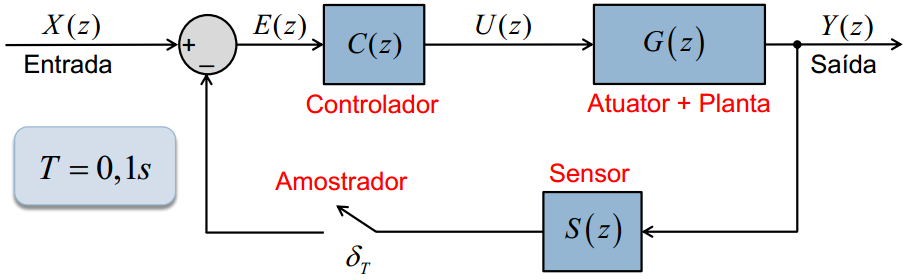
\includegraphics[scale = .5]{Imagens/Execicio1_pr2.PNG}
    \caption{Diagrama de blocos da prática 2.}
    \label{fig:pr2_esquema}
\end{figure}

\section{Resultados e discussões}

Realizando o equacionamento genérico a malha fechada do sistema apresentado na Figura \ref{fig:pr2_esquema} encontra-se a equação (\ref{pr_2_3})  
\begin{equation}
\frac{Y(z)}{X(z)} = \frac{C(z)G(z)}{1 + C(z)G(z)S(z)}
\label{pr_2_3}
\end{equation}

Substituindo as equações (\ref{pr_2_C}), (\ref{pr_2_G}) e (\ref{pr_2_S}) na equação (\ref{pr_2_3}) e expressado com a razão polinomial de $z^{-1 }$ temos

\begin{equation}
\frac{Y(z)}{X(z)} = \frac{0,27z^{-1} - 0,216z^{-2}}{1 - 1,7z^{-1} + 0,854z^{-2} - 0,1z^{-3}}
\label{pr_2_4}
\end{equation}

Através da equação (\ref{pr_2_4}) aplica-se o método da equação de diferença conforme apresentado na equação (\ref{pr_2_2}), concebendo a equação (\ref{pr_2_5}) que será simulada com o respectivo sinal de entrada.

\begin{equation}
y(k) =  1,7y(k-1) - 0,854y(k-2) + 0,1y(k-3) + 0,27x(k-1) - 0,216x(k-2)
\label{pr_2_5}
\end{equation}

O código implementado em Matlab está mostrado abaixo:
\lstinputlisting{Arquivos_tex/Aula_5_Exercicio_2.m}

Obtendo como saída o gráfico da Figura \ref{saida_ex2_pr_2}.

\begin{landscape}
  \begin{figure}[!ht]
      \centering
      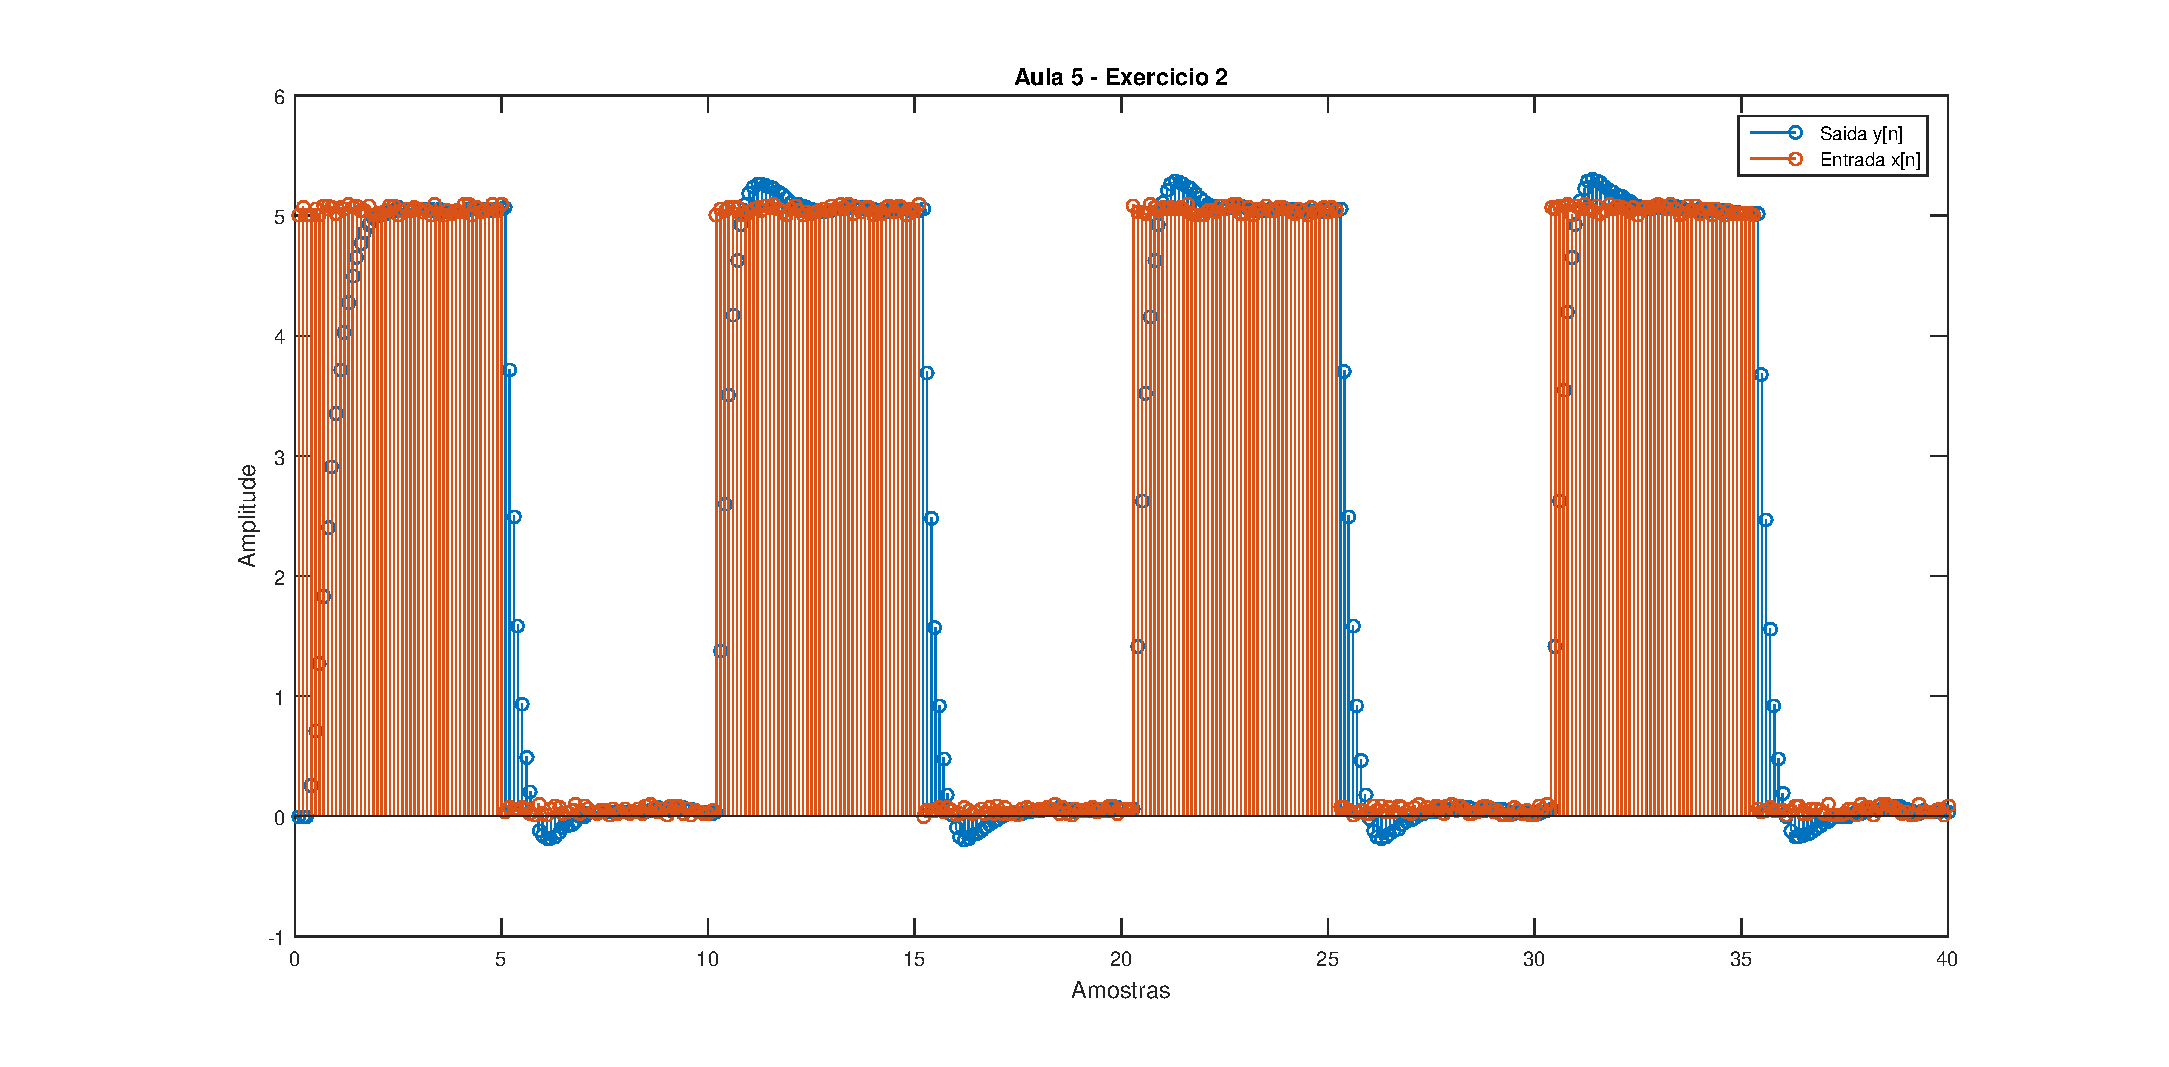
\includegraphics[scale = .66]{Imagens/Aula_5_exercicio2.eps}
      \caption{Gráfico de saída do código do exercício da prática 2.}
      \label{saida_ex2_pr_2}
  \end{figure}
\end{landscape}

A transformada $z$ é uma ferramenta comumente utilizada para análise e síntese de sistemas de controle em tempo discreto. Análoga a transformada de Laplace, possui a equação de diferenças como ferramenta matemática para a obtenção da resposta do sistema a uma dada entrada. 

Como a natureza exprime sistemas variáveis no tempo de forma contínua, a transformada inversa $z$ permitiu através do método de equações de diferenças fornece a saída em tempo discreto fazendo uso do tempo de amostragem que simule um sistema pseudo-contínuo.

Este método recursivo possibilitou a implementação digital, conforme o exercício apresentado, de forma simplista utilizando laço de controle e vetores. Na Figura \ref{saida_ex2_pr_2}, dado a entrada de uma onda quadrada, o PID, a planta e o sensor interagem na malha fornecendo uma resposta com baixo sobresinal e rápido tempo de assentamento.